\section{Theoretical Analysis}
\label{sec:analysis}

In this section, the circuit shown in Figure \ref{fig:t2} is analysed
theoretically, in terms of each branch's current and voltage.
The current flows considered in the analysis are the following:
$R_1$ from node 1 to 2; $R_2$ from node 2 to 3; $R_3$ from node 2 to 4; $R_4$ from node 4 to 0; $R_5$ from node 4 to 5; $R_6$ from node 0 to 6; $R_7$ from node 6 to 7. Also, the potencial in Node 0 was considered to be 0V (ground). Node 8 is an auxiliary node which is going to be needed in the simulation.

\subsection{Nodal Analysis for t$<$0}

In this first step, we use Nodal Analysis to determine the voltage in each node as well as the current in every branch of the circuit, when t$<$0. \par 
This method is based on Kirchhoff's Current Law (KCL), and firstly consists in
deriving equations for the current flow in nodes not connected to voltage sources,
followed by writing aditional equations in nodes related to voltage sources. The node 
identification can be seen on Figure \ref{fig:t2}. Moreover, the equations relative to
nodes 0, 0, 2, 3 and 5, respectively, are

\begin{equation}
  (V_0 - V_4)/R_4 + (V_0 - V_6)/R_6 + (V_1 - V_2)/R_1 = 0 
  \label{eq:kvl1}
\end{equation}

\begin{equation}
  (V_6 - V_7)/R_7 + (V_0 - V_4)/R_4 + (V_1 - V_2)/R_1 = 0 
  \label{eq:kvl2}
\end{equation}

\begin{equation}
  (V_2 - V_1)/R_1 + (V_2 - V_4)/R_3 + (V_2 - V_3)/R_2 = 0
  \label{eq:kvl3}
\end{equation}

\begin{equation}
  (V_3 - V_2)/R_2 = K_b(V_2 - V_4)
  \label{eq:kvl4}
\end{equation}

\begin{equation}
  (V_4 - V_5)/R_5 = K_b(V_2 - V_4)
  \label{eq:kvl5}
\end{equation}

The aditional equations for the method are

\begin{equation}
  V_4 - V_7 = K_d(V_0 - V_6)/R_6
  \label{eq:kvl6}
\end{equation}

\begin{equation}
  V_0 = 0
  \label{eq:kvl7}
\end{equation}

\begin{equation}
  V_1 = V_s
  \label{eq:kvl8}
\end{equation}


\begin{table}[h]
  \centering
  \begin{tabular}{|l|r|}
    \hline    
    {\bf Name} & {\bf Value [A or V]} \\ \hline
    $I_b$ & -2.658976e-04
$I_c$ & 0
$I_R$$_1$ & 2.536488e-04
$I_R$$_2$ & 2.658976e-04
$I_R$$_3$ & -1.224882e-05
$I_R$$_4$ & 1.205310e-03
$I_R$$_5$ & -2.658976e-04
$I_R$$_6$ & 9.516615e-04
$I_R$$_7$ & 9.516615e-04
$V_1$ & 5.054819
$V_2$ & 4.793705
$V_3$ & 4.258198
$V_4$ & 4.831047
$V_5$ & 5.668298
$V_6$ & -1.934226
$V_7$ & -2.905231
$V_8$ & -1.934226

  \end{tabular}
  \caption{Nodal Analysis' variable values for t$<$0, where $I_j$ is expressed in Ampere and $V_j$ is expressed in Volt.}
  \label{tab:Nodal}
\end{table}
\FloatBarrier

\subsection{Equivalent resistance $R_{eq}$}
\label{sec:2.2}

In this step, we use the previously computed values to calculate a voltage defined as $V_x$ = $V_5$ - $V_7$ (voltages in nodes 5 and 7, respectively - which correspond to nodes 6 and 8 from the laboratory paper). Note that this is the voltage drop at the capacitor's terminals, which will be needed for further analysis of the circuit. Firstly, we make $V_S$ = 0. Then, by running nodal analysis again, we can obtain the current $I_x$ flowing through $V_x$. With both these values computed, we can now obtain the value of the equivalent resistance $R_{eq}$ as seen by the capacitor, which is given by $R_{eq}$ = $V_x$/$I_x$. Finally, we can also compute the time constant $\tau$ given by $\tau$ = $R_{eq}$C. Also, this corresponds to the initial calculations for computing the natural solution. \par
Defining $V_x$ = $V_5$ - $V_7$ makes sense because the voltage drop in the capacitor is a continuous function, so $V_x$(t$<$0) = $V_x$(t=0).
We considered the equations \ref{eq:kvl1}, \ref{eq:kvl2}, \ref{eq:kvl3}, \ref{eq:kvl4}, \ref{eq:kvl6}, \ref{eq:kvl7} and the following two:

\begin{equation}
  V_5 - V_7 = V_x
  \label{eq:kvl9}
\end{equation}

\begin{equation}
 V_1 = V_s 
  \label{eq:kvl10}
\end{equation}


\begin{table}[h]
  \centering
  \begin{tabular}{|l|r|}
    \hline    
    {\bf Name} & {\bf Value [A or V or $\Omega$ or s]} \\ \hline
    $I_b$ & 0.000000
$I_R$$_1$ & 0.000000
$I_R$$_2$ & 0.000000
$I_R$$_3$ & 0.000000
$I_R$$_4$ & 0.000000
$I_R$$_5$ & -2.722816e-03
$I_R$$_6$ & -0.000000
$I_R$$_7$ & 0.000000
$V_1$ & 0.000000
$V_2$ & 0.000000
$V_3$ & 0.000000
$V_4$ & 0.000000
$V_5$ & 8.573530
$V_6$ & 0.000000
$V_7$ & 0.000000
$V_8$ & 0.000000
$V_X$ & 8.573530
$I_X$ & -2.722816e-03
$R_e$$_q$ & -3148.773562
$tau$ & -3.239206e-03
$I_b$ & 0.000000
$I_R$$_1$ & 0.000000
$I_R$$_2$ & 0.000000
$I_R$$_3$ & 0.000000
$I_R$$_4$ & 0.000000
$I_R$$_5$ & -2.722816e-03
$I_R$$_6$ & -0.000000
$I_R$$_7$ & 0.000000
$V_1$ & 0.000000
$V_2$ & 0.000000
$V_3$ & 0.000000
$V_4$ & 0.000000
$V_5$ & 8.573530
$V_6$ & 0.000000
$V_7$ & 0.000000
$V_8$ & 0.000000
$V_X$ & 8.573530
$I_X$ & -2.722816e-03
$R_e$$_q$ & -3148.773562
$tau$ & -3.239206e-03
$I_b$ & 0.000000
$I_R$$_1$ & 0.000000
$I_R$$_2$ & 0.000000
$I_R$$_3$ & 0.000000
$I_R$$_4$ & 0.000000
$I_R$$_5$ & -2.722816e-03
$I_R$$_6$ & -0.000000
$I_R$$_7$ & 0.000000
$V_1$ & 0.000000
$V_2$ & 0.000000
$V_3$ & 0.000000
$V_4$ & 0.000000
$V_5$ & 8.573530
$V_6$ & 0.000000
$V_7$ & 0.000000
$V_8$ & 0.000000
$V_X$ & 8.573530
$I_X$ & -2.722816e-03
$R_e$$_q$ & -3148.773562
$tau$ & -3.239206e-03

  \end{tabular}
  \caption{Equivalent resistance $R_{eq}$ and time constant $\tau$}
  \label{tab:Req}
\end{table}
\FloatBarrier

\subsection{Natural Solution}

Now, using the previous results we can compute the natural solution $v_{5n}$(t) from 0 to 20ms in time, as requested. We know that the solution is of the general form 
\begin{equation}
Ae^{-t/\tau}.
\label{eq:kvl11}
\end{equation}

Now, we only need an initial condition to find the constant "A" which is going to be the value of $V_x$, the capacitor's voltage for t$\leq$0. A plot of the solution in t$\in$[0;20]ms is shown in \ref{fig:v5_n}. Analysing the parameters of the circuit for t=0 we note that $V_7$ = 0V and $V_c$ decreases, which leads to

\begin{equation}
  V_5 = V_c = V_xe^{t/\tau} 
  \label{eq:kvl12}
\end{equation}


\begin{figure}[h] \centering
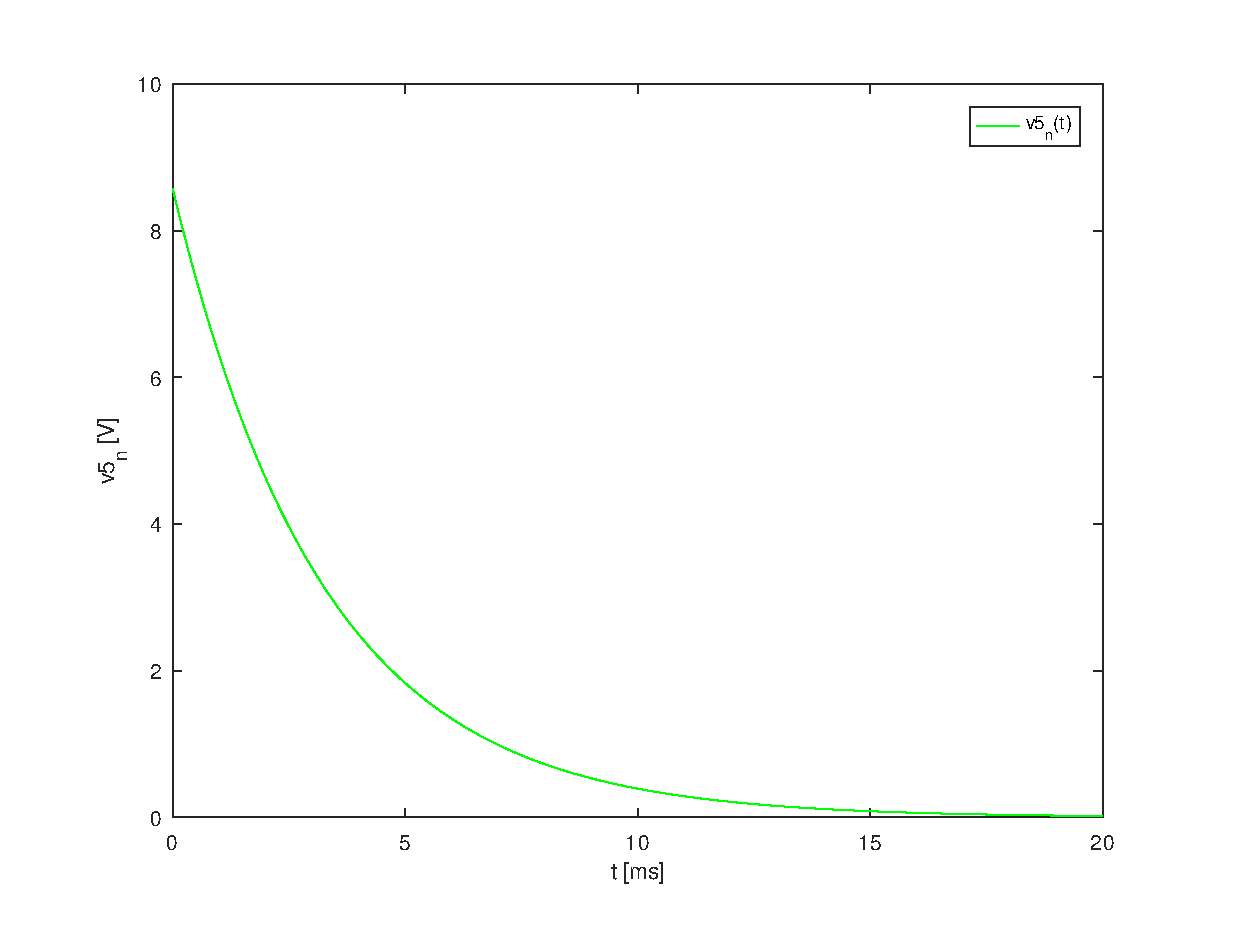
\includegraphics[width=0.6\linewidth]{v5_n.eps}
\caption{Natural solution for $v_5$}
\label{fig:v5_n}
\end{figure}
\FloatBarrier

\subsection{Forced solution}

In this step, we use a phasor voltage source $V_S$ and replace the capacitor with its impedance $Z_C$. Then we use the nodal method again in order to determine the phasor voltages in every node, and register the data in \ref{tab:Phasors}. \par
The goal is to obtain the forced solution $v_{5f}$(t) in t$\in$[0;20]ms for a frequency f = 1kHz. \par
The nodal analysis is equivalent to the previous ones in terms of equations, but instead of voltages we use phasors:

%Aqui aplicou-se o método dos nós, mas temos phasors, portanto repetirei todas as eqs mas assinalo as que ficam diferentes caso queiram tirar as que estão a mais

\begin{equation}
  (\tilde{V}_2 - \tilde{V}_1)/R_1 + (\tilde{V}_2 - \tilde{V}_4)/R_3 + (\tilde{V}_2 - \tilde{V}_3)/R_2 = 0
  \label{eq:4_13}
\end{equation}

\begin{equation}
 (\tilde{V}_0 - \tilde{V}_4)/R_4 + (\tilde{V}_0 - \tilde{V}_6)/R_6 + (\tilde{V}_1 - \tilde{V}_2)/R_1 = 0 
  \label{eq:4_14}
\end{equation}

\begin{equation}
  (\tilde{V}_6 - \tilde{V}_7)/R_7 + (\tilde{V}_0 - \tilde{V}_4)/R_4 + (\tilde{V}_1 - \tilde{V}_2)/R_1 = 0 
  \label{eq:4_15}
\end{equation}

\begin{equation}
  (\tilde{V}_3 - \tilde{V}_2)/R_2 = K_b(\tilde{V}_2 - \tilde{V}_4)
  \label{eq:4_16}
\end{equation}

\begin{equation}
  (\tilde{V}_5 - \tilde{V}_7)/Z_C + (\tilde{V}_5 - \tilde{V}_4)/R_5 + K_b(\tilde{V}_2 - \tilde{V}_4) = 0, Z_C = 1/(jwC)
  \label{eq:4_17}
\end{equation}

\begin{equation}
  \tilde{V}_4 - \tilde{V}_7 = K_d(\tilde{V}_0 - \tilde{V}_6)/R_6
  \label{eq:kvl18}
\end{equation}

\begin{equation}
  \tilde{V}_1 = \tilde{V}_s
  \label{eq:kvl19}
\end{equation}


\begin{figure}[h] \centering
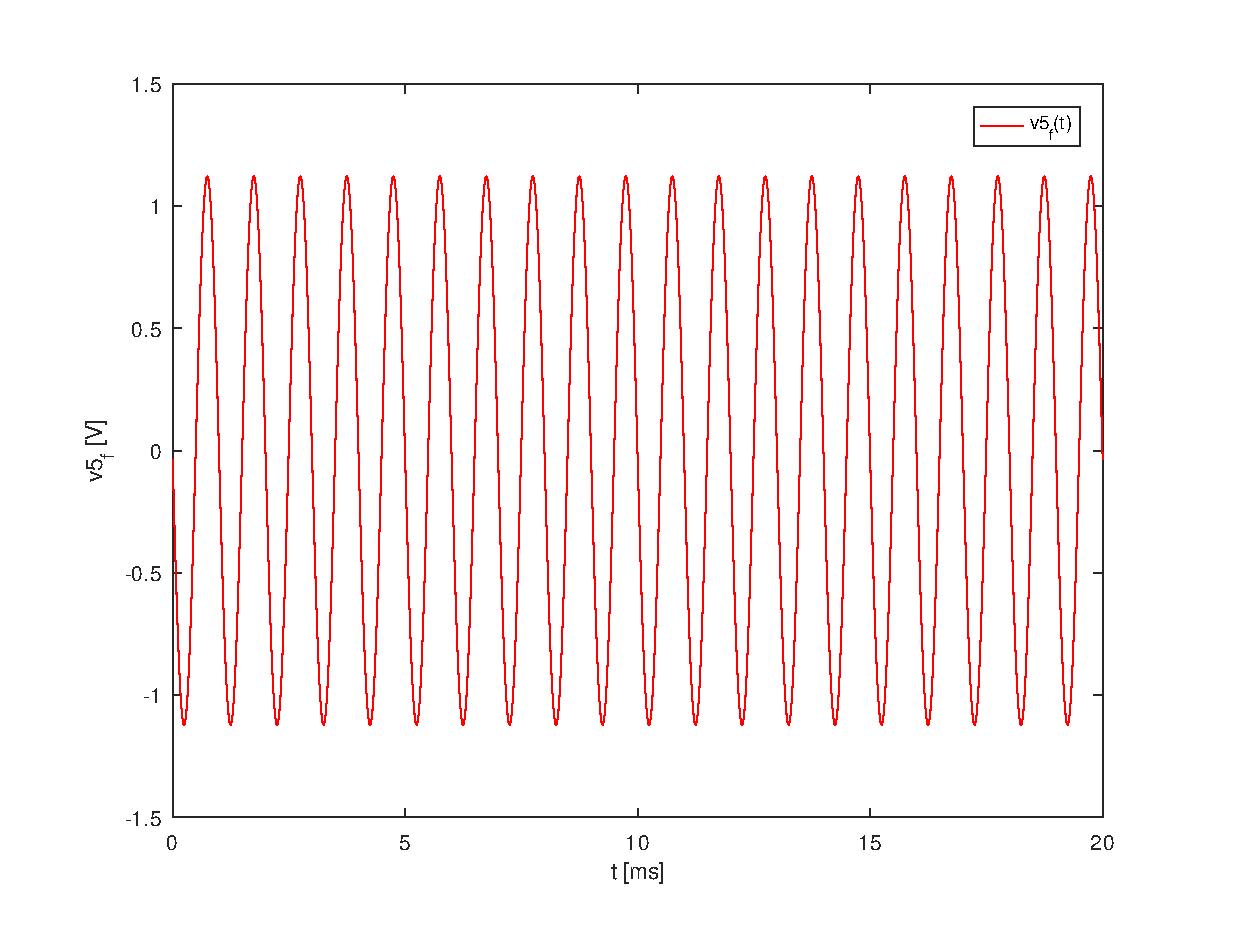
\includegraphics[width=0.6\linewidth]{v5_f.eps}
\caption{Forced Solution for $v_5$}
\label{fig:v5_f}
\end{figure}
\FloatBarrier


\begin{table}[h]
  \centering
  \begin{tabular}{|l|r|}
    \hline    
    {\bf Name} & {\bf Value [V]} \\ \hline
    $V_1$ & 1.000000
$V_2$ & 0.948344
$V_3$ & 0.842404
$V_4$ & 0.955731
$V_5$ & 1.121194
$V_6$ & 0.382650
$V_7$ & 0.574745
$V_8$ & 0.382650

  \end{tabular}
  \caption{Complex amplitudes in the nodes}
  \label{tab:Phasors}
\end{table}
\FloatBarrier



\subsection{Final solution}

Now we are able to describe the final solution $v_5$(t) after converting the forced solution to a real time function. The solution is the sum of the contributions of the natural and forced responses of the circuit:  

\begin{equation}
  v_5 = v_{5f} + v_{5n}
  \label{eq:kvl20}
\end{equation}

\begin{figure}[h] \centering
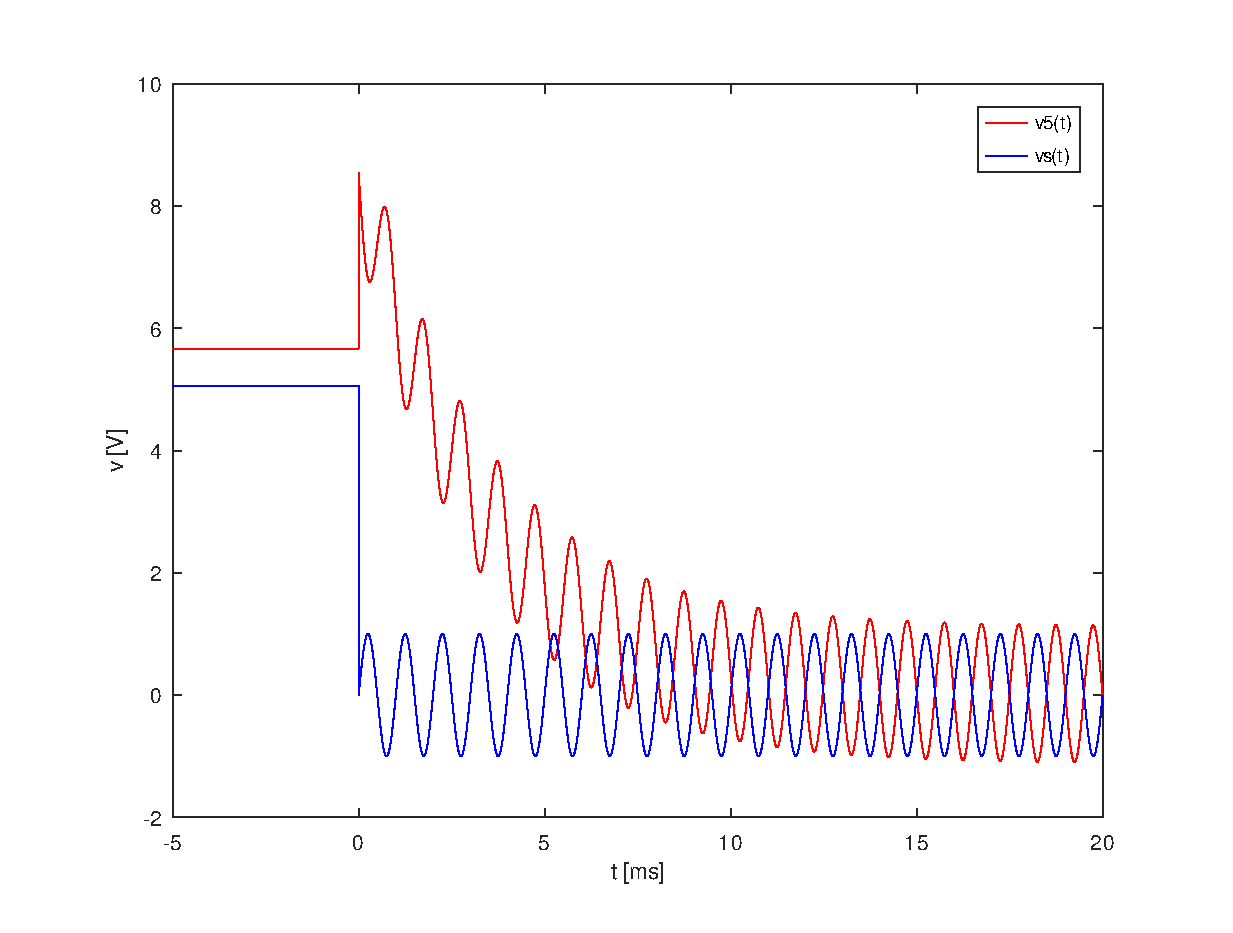
\includegraphics[width=0.6\linewidth]{v5_vs.eps}
\caption{Final Solution for $v_5$ and $v_s$}
\label{fig:v5_vs}
\end{figure}
\FloatBarrier

\subsection{Frequency response}

In this final step we use the functions $v_5$(f) and $v_7$(f) (voltages on nodes 5 and 7, respectively, in terms of frequency, f) using a logarithmic scale for frequency (dB) and expressing the phase in degrees, with f$\in$[0.1;1]kHz. \par
Defining $v_C$(f) = $v_5$(f) - $v_7$(f), we can then plot different functions $v_S$(f), $v_C$(f) and $v_6$(f) as seen in \ref{fig:freqresp} (amplitude) and in \ref{fig:phase_oct} (phase, in degrees).

%EXPLICAR AS DIFERENÇAS

\begin{figure}[h] \centering
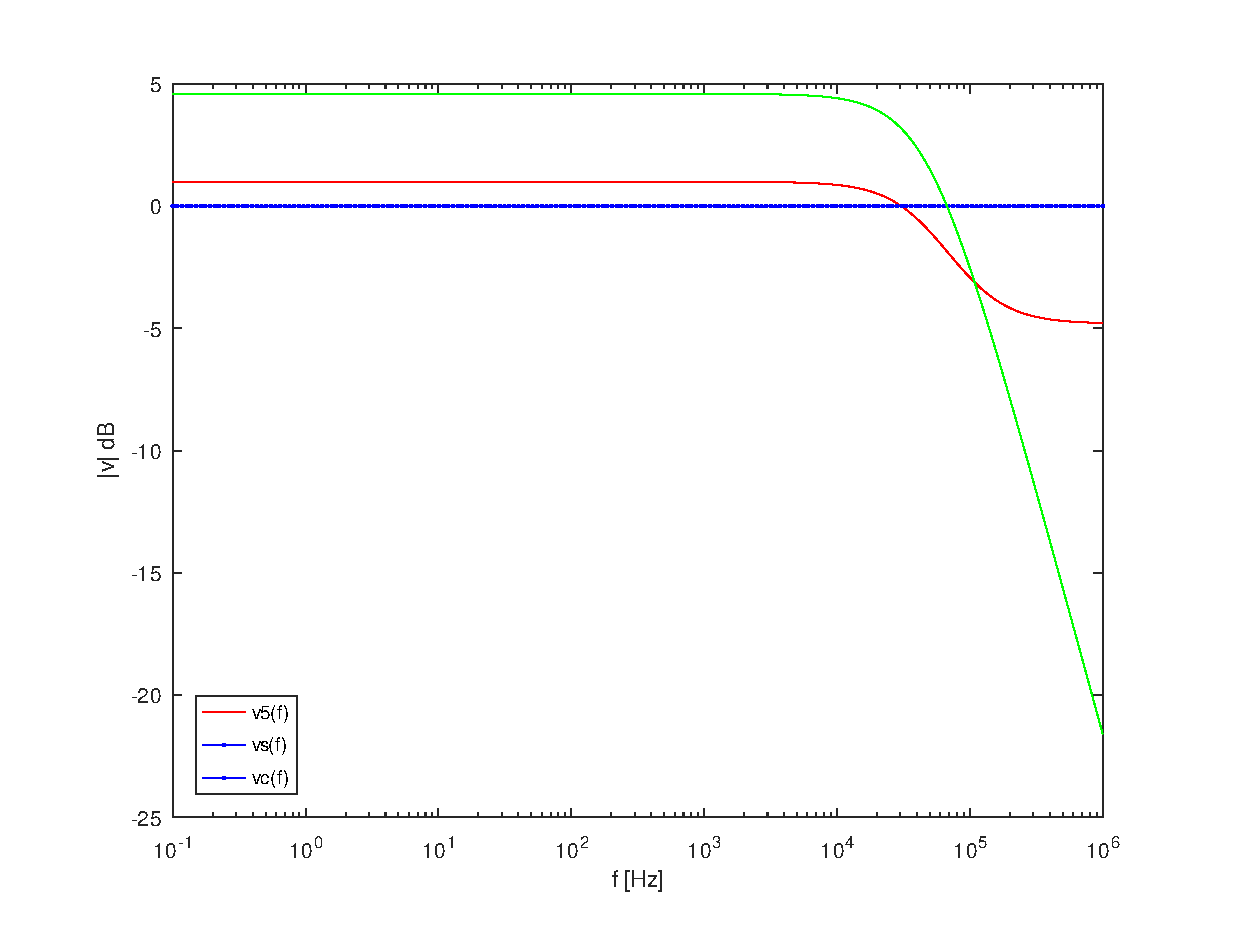
\includegraphics[width=0.6\linewidth]{freqresp.eps}
\caption{Magnitude in dB $v_5$(f) (red), $v_s$(f) (blue), $v_c$(f) (green)}
\label{fig:freqresp}
\end{figure}
\FloatBarrier

\begin{figure}[h] \centering
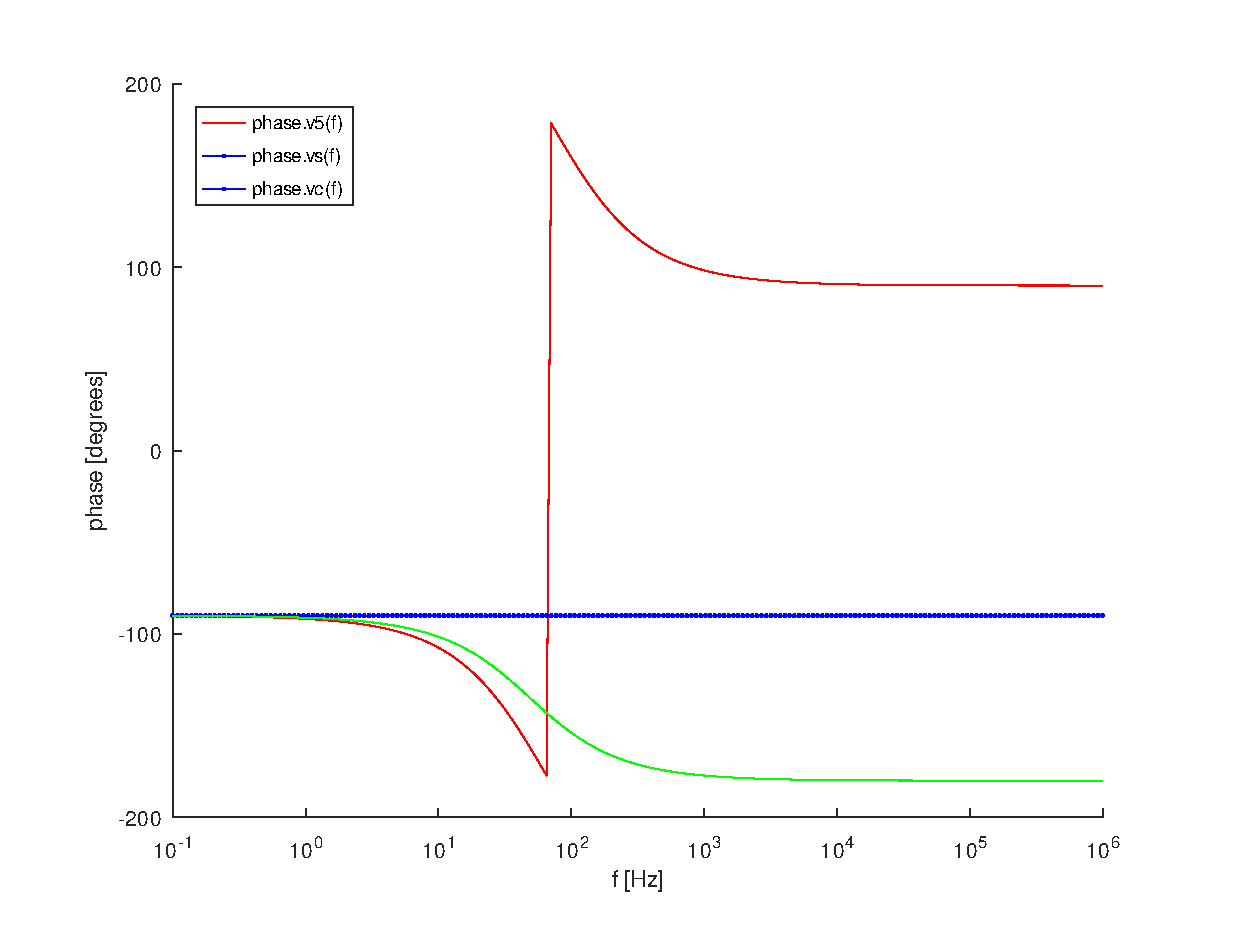
\includegraphics[width=0.6\linewidth]{phase_oct.eps}
\caption{Phase in degrees $v_5$(f) (red), $v_s$(f) (blue), $v_c$(f) (green)}
\label{fig:phase_oct}
\end{figure}
\FloatBarrier

















